



\chapter{Activity in Brownian Motion}

\section{Introduction}
The final part of this manuscript is dedicated to the study of active matter and its interplay with Brownian motion. This subject was actually the motivation for my PhD thesis, and the first part of this Chapter is dedicated to my first introduction to the field of active matter. I begin with a full introduction to what Active matter is, and how it is typically modeled in the most popular algorithms. 

The second part, which came much later in my PhD, treats the problem of active Taylor-Aris dispersion. The notion of Taylor-Aris dispersion is described in the previous Chapter. For the sake of clarity, I thus invite the reader to consult its developments before reading this part. We conducted this work in tandem with Marc Lagoin, Guirec de Tournemire, Ahmad Badr and Antoine Allard, and published it in PNAS. 
\subsection{Activity}

Authors define active matter as one or both of the following:

\begin{enumerate}
    \item "energy-consuming particles" : individual units that extract free energy from internal or external sources and convert it to motion, forces, or mechanical stresses (this is the definition I use in this manuscript) . This work is not necessarily expressed in the form of self-propelling \cite{prost_active_2009}\cite{ramaswamy_active_2010}\cite{marchetti_hydrodynamics_2013} \cite{bechinger_active_2016}. They are thus inherently out-of-equilibrium systems;
    \item "interacting particles" : individual self-propelled units which interact locally and exhibit emergent, collective behaviour, such as 
    hydrodynamic interactions (swimming microorganisms, squirmers, active droplets...)\cite{marchetti_hydrodynamics_2013}, phoretic interactions (catalytic Janus colloids, some chemotactic bacteria...)\cite{palacci_living_2013}, mechanical force transmission (cellular tissue, cytoskeleton, active gels...)\cite{prost_active_2009}, and even social interactions (human crowds, bird flocks, fish schools, autonomous drones...)\cite{toner_hydrodynamics_2005}, to only cite a few. Some of these interactions can be accurately represented with minimal models, which approximate them as alignment interactions with some noise, such as the Vicsek model \cite{vicsek_novel_1995}. Certain authors distinguish these instances of interacting active matter from the first I mentioned \cite{bechinger_active_2016}.
\end{enumerate}



 

Numerous examples of active systems exist, and these systems can be found at any scale (Fig. \ref{Reynolds_sizes}). I find it convenient to not only classify them by size but also by typical Reynolds number, as most of them will typically use their surrounding energy source to move in space.Interestingly, the definition of active matter is loose enough to even include human beings, robots and even large aircrafts.  This thesis articulates around notions of small systems, and I thus refer to these systems form there on.

We may for example cite the very famous example of \emph{Chlamydomonas Reinhardtii}. These tiny algae will be the basis of our publication at the end of this Chapter. They measure only a few tens of microns at most. However, through the beating of the flagella at their front, they are able to self-propel in a fluid at the surprisingly high speed of ten body lengths per second. Yet, this is not sufficient for \emph{Chlamydomonas} to be considered high-Reynolds systems ($R_\mathrm{e} \gg 1$), as they typically reach a Reynolds number of about $R_\mathrm{e} = 1 \times 10 ^{-4}$. They thus still evolve in a very viscous medium. Furthermore, these algae are able to orient towards or away from light sources through the use of an eye spot, which is able to sense both a light's wavelength and its intensity. Under certain conditions, their behaviour may completely change from a swimmer with random and erratic reorientations, to phototactic, to a glider, stuck to the boundary of its observation box, and only slowly moving in its sticking plane.



\begin{figure}
    \centering
    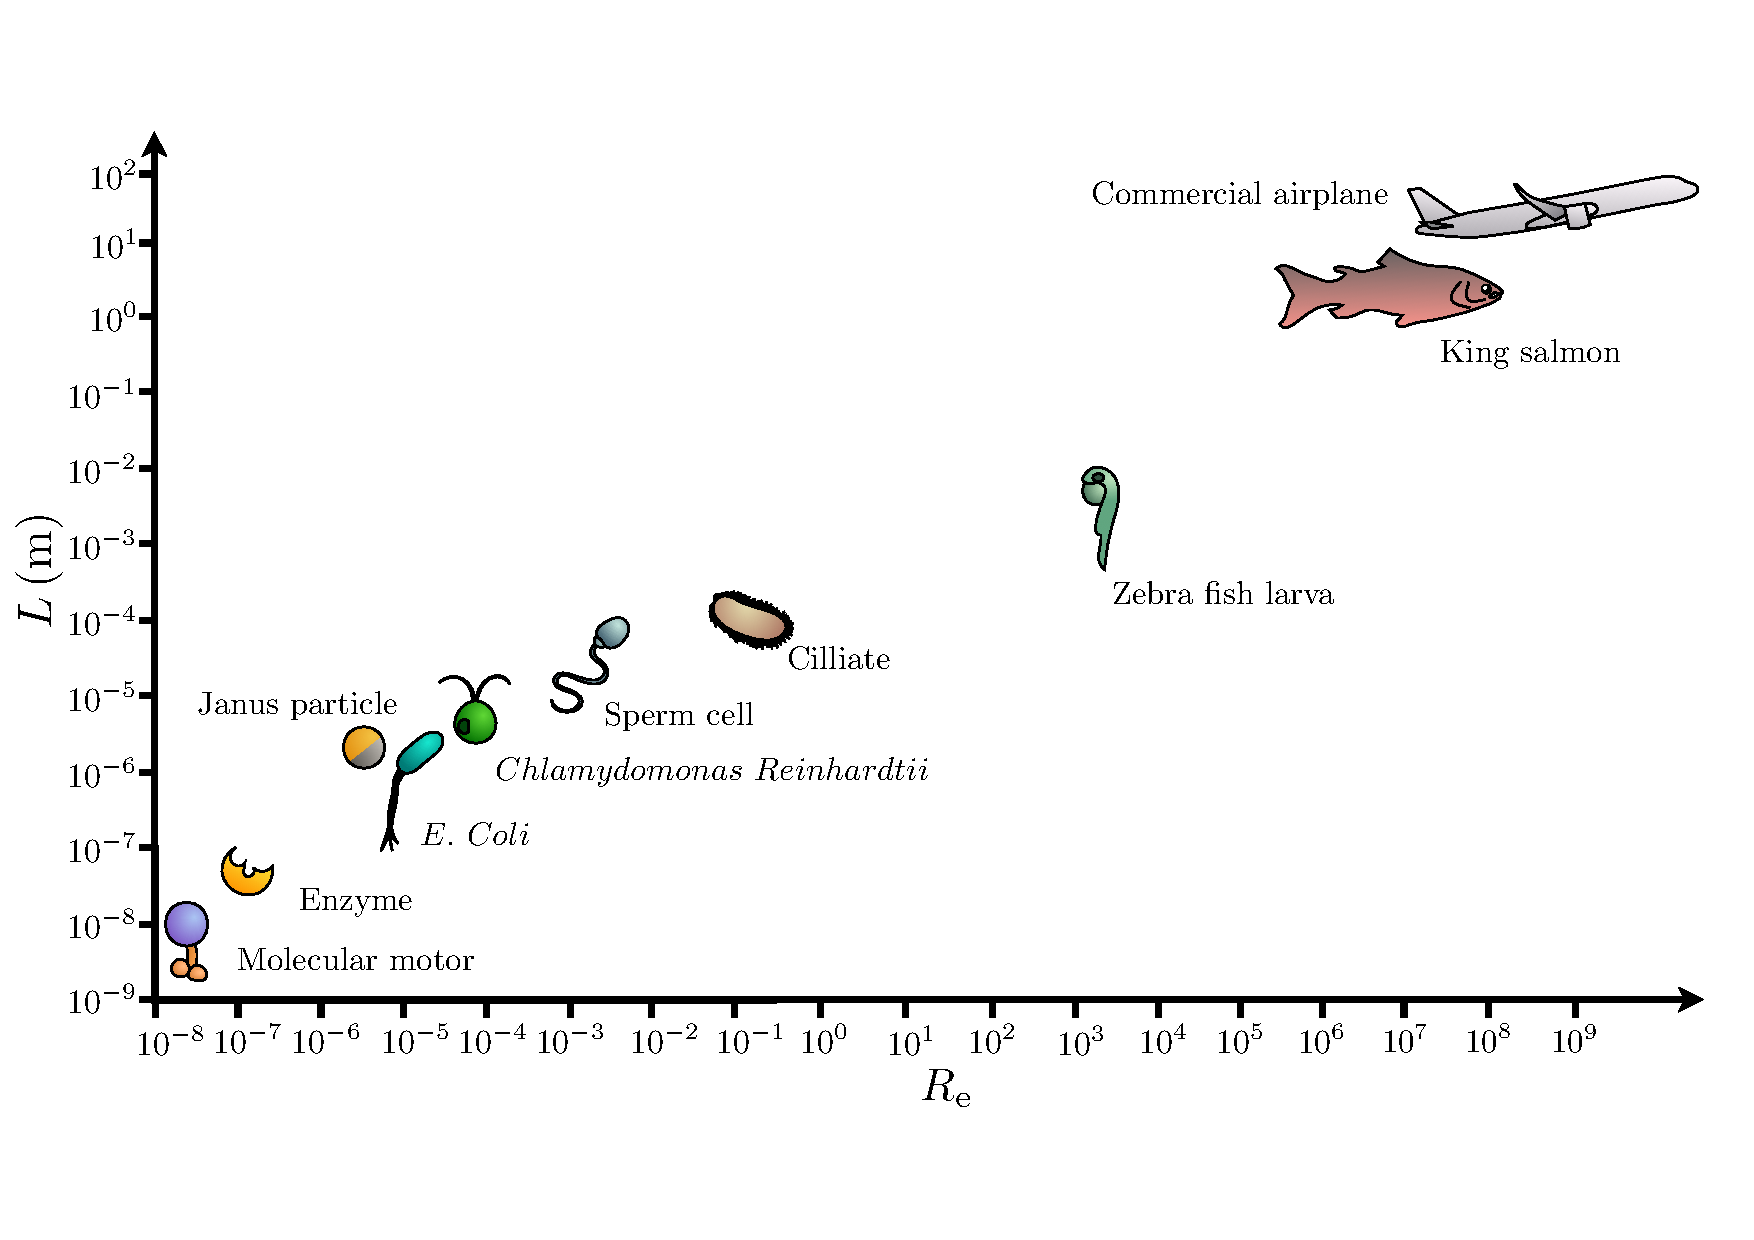
\includegraphics[width=1\textwidth]{figures/chapter5/fig1.pdf}
    \caption{Comparison of typical length scales and Reynolds numbers for various active systems. }
    \label{Reynolds_sizes}
\end{figure}




\section{Classes of microswimmers}

\subsection{Biological swimmers}


\subsection{Artificial swimmers}


\section{Modelling approaches}
Multiple techniques exist to simulate active matter. I describe here the ones I have come to know or use during my thesis, starting with non-interacting simulations (ABPs, RNTs, chiral ABPs) \cite{bechinger_active_2016}. 
I also provide in appendix and on the GitHub repository \textcolor{red}{ADD GITHUB} a simple Jupyter file to simulate ABPs, RNTs and to compare them to the passive case. This file also contains a very small exploration of chiral Brownian particles.  

\subsection{Active Brownian Particles}
For comparison purposes, let us recall that a purely passive colloid undergoes thermal diffusion. This thermal diffusion affects both the translational degrees of freedom ($x$ and $y$ for a two-dimensional case) and the rotational degree of freedoms ($\phi$ for a two-dimensional case). We define from the Stokes-Einstein relation the translational thermal diffusion coefficient $D_\mathrm{T}$ as:


\begin{equation}
D_\mathrm{T} = \frac{k_\mathrm{B}\Theta}{6\pi \eta a}~,
\label{ThermalD}
\end{equation}
where $k_\mathrm{B}\Theta$ is the thermal energy of the bath, $\eta$ the fluid visicosity and $a$ the colloid radius. The rotational diffusion coefficient $D_\mathrm{R}$, however, is proportional to the colloid's volume:
\begin{equation}
D_\mathrm{R} = \frac{k_\mathrm{B}\Theta}{8\pi \eta a^3 }= \tau_\mathrm{R}^{-1}~,
\label{ActiveR}
\end{equation}
with $\tau_\mathrm{R}$ a characteristic reorientation timescale.

We have already stated that we can describe the motion of the passive colloid with the following Langevin equations for the overdamped limit:

\begin{equation}
\label{PassiveBrownian}
\begin{aligned}
   \frac{\mathrm{d}x}{\mathrm{d}t} &= \sqrt{2D_\mathrm{T}}\xi_x(t) \\
   \frac{\mathrm{d}y}{\mathrm{d}t} &= \sqrt{2D_\mathrm{T}}\xi_y(t) \\
   \frac{\mathrm{d}\phi}{\mathrm{d}t} &= \sqrt{2D_\mathrm{R}}\xi_\phi(t)~.
\end{aligned}
\end{equation}
where $\xi_i(t)$ white Gaussian noises of correlation $\delta (t)$. This process is heavily reliant on the thermal diffusion coefficients $D_\mathrm{T}$ and $D_\mathrm{R}$, which are themselves proportional to temperature and inversely proportional to colloid radius and fluid viscosity. This means that thermal Brownian motion is strongly hindered in the case of larger colloids, where larger means of the order of a few tens of microns. For example, if we take for comparison with later cases a colloid of a size that is comparable to a \emph{Chlamydomonas}, that is to say $a = 10 \upmu \mathrm{m}$, we get $D_\mathrm{T}=2.2\times10^{-3}\upmu \mathrm{m}^2.\mathrm{s}^{-1}$. We interpret that by pure thermal diffusion, a colloid of this size would need tens of hours to explore an area equivalent to its own size.

Lucky, as we discussed already, swimmers circumvent this limitation by collecting energy from their surroundings to self propel amongst other strategies. A very simple model used to represent a swimmer with an ability to self-propel with a given velocity $\vec{v}$ is the Active Brownian Particle (APB) model. We describe this model with the following Langevin equations:
\begin{equation}
\begin{aligned}
    \label{ActiveBrownian}
    \frac{\mathrm{d}x}{\mathrm{d}t} &= v \cos[\phi(t)] + \sqrt{2D_\mathrm{T}}\xi_x(t)\\
    \frac{\mathrm{d}y}{\mathrm{d}t} &= v\sin[\phi(t)] + \sqrt{2D_\mathrm{T}}\xi_y(t)\\
    \frac{\mathrm{d}\phi}{\mathrm{d}t} &= \sqrt{2D_\mathrm{R}}\xi_\phi(t)~.
\end{aligned}
\end{equation}
We notice that the swimmer is still undergoing thermal diffusion for the rotational degree of freedom, with a characteristic time $\tau_\mathrm{R}$ after which the swimmer "forgets" in which direction it was heading. This memory effect can be noticed at very short times 



\begin{figure}
    \centering
    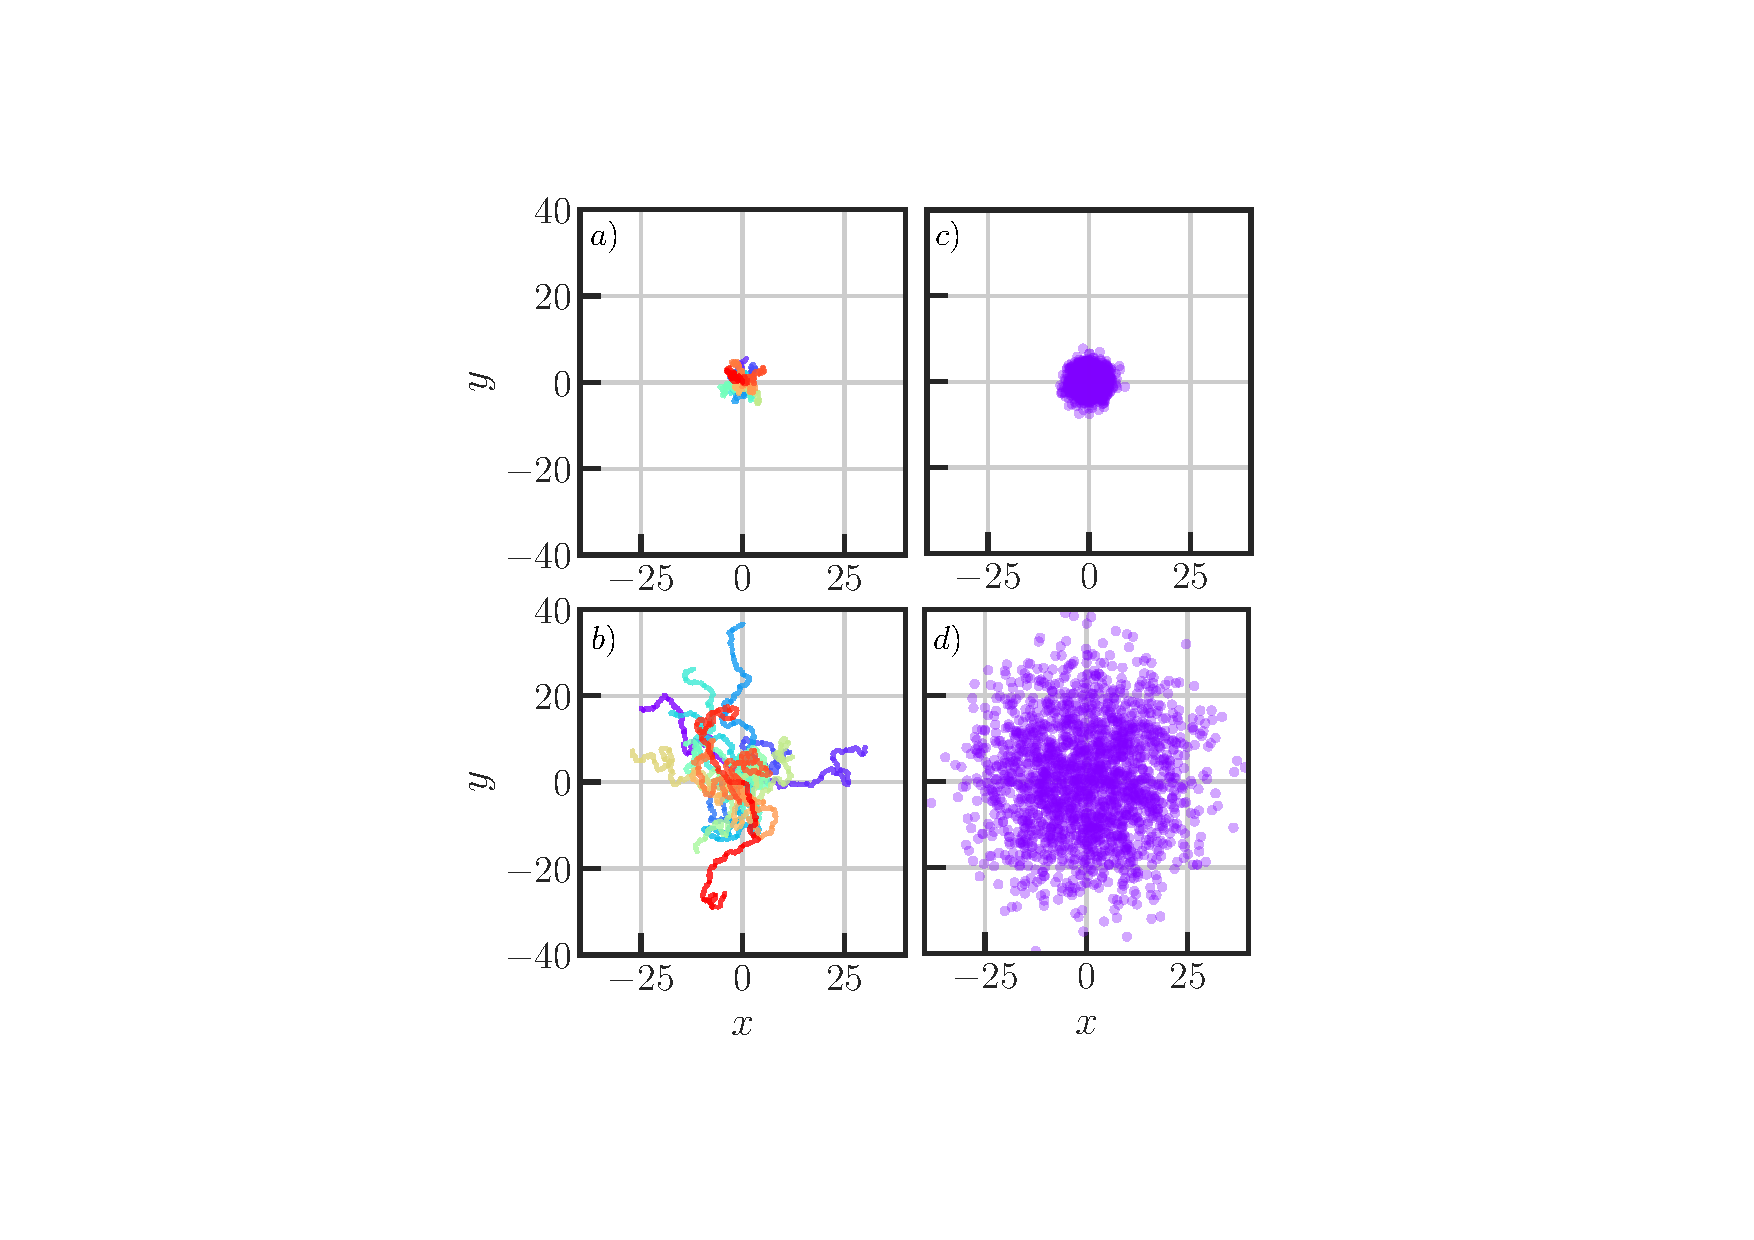
\includegraphics[width=.5\textwidth]{figures/chapter5/compaABP_PBP.pdf}
    \caption[Simulation of passive BM and ABP models.]{Comparison of passive and active Brownian colloid trajectories. Panels \textbf{a)} and \textbf{c)}: Twenty stacked trajectories obtained from discretising Eqs. \ref{PassiveBrownian} and \ref{ActiveBrownian} respectively, with $\Delta t = 0.05$, $n_\mathrm{steps} = 5000$, $D_\mathrm{T} = 0.05$, $D_\mathrm{R} = 0.3$, $v = 0.1$, with all units in simulation units. Colours are only used for readability and have no physical meaning. Panels \textbf{c)} and \textbf{d)}: final position of 2000 simulations for the passive and active Brownian particle models, respectively. }
    \label{ABPPBP}
\end{figure}





\begin{tabular}{lccc}
\hline
Case & $D_\mathrm{T}$ & Persistence time & $D_\mathrm{eff}$ \\
\hline
Passive BM ($a=0.5\,\mu$m) & 0.44 & -- & 0.44 \\
ABP ($a=0.5\,\mu$m) & 0.44 & 0.77 s & 0.82 \\
Passive BM ($a=10\,\mu$m) & $2.2\times10^{-2}$ & -- & $2.2\times10^{-2}$ \\
ABP ($a=10\,\mu$m) & $2.2\times10^{-2}$ & 6250 s & $3.0\times10^3$ \\
\hline
\end{tabular}




\subsubsection{Chiral ABPs}

Some microswimmers or clusters of microswimmers have irregular shapes or asymmetrical propulsion mechanisms.

While the ABP translation mechanisms remain unchanged, one can introduce chiral behaviour in the ABP model by adding a constant rotation speed $\omega$ in the angular Langevin equation, as follows:
\begin{equation}
\begin{aligned}
    \label{ActiveBrownian}
    \frac{\mathrm{d}x}{\mathrm{d}t} &= v \cos[\phi(t)] + \sqrt{2D_\mathrm{T}}\xi_x(t)\\
    \frac{\mathrm{d}y}{\mathrm{d}t} &= v\sin[\phi(t)] + \sqrt{2D_\mathrm{T}}\xi_y(t)\\
    \frac{\mathrm{d}\phi}{\mathrm{d}t} &=\omega  \sqrt{2D_\mathrm{R}}\xi_\phi(t)~.
\end{aligned}
\end{equation}
It is therefore possible to play with the phase to obtain different behaviours, from shrinking spirals to circles to expanding spirals for the two-dimensional case.

Helical motion can be described using a three-dimensional ABP model, such as
\begin{align}
\frac{\mathrm d \mathbf r}{\mathrm dt} &= v \mathbf{n} + \sqrt{2D_t}\,\boldsymbol{\xi_\mathrm{T}}(t),\\
\frac{\mathrm d \mathbf n}{\mathrm dt} &= \boldsymbol{\Omega}\times\mathbf{n}+ \sqrt{2D_r}\,
\boldsymbol{\xi_\mathrm{R}}(t)\times\mathbf{n},
\label{3d_helical}
\end{align}

with $\mathbf{r}$ the position vector $ \mathbf{r} = (x,y,z)$, and $\mathbf{n}$ the orientation vector, which must be normalised, as $ \mathbf{n} = (n_x,n_y,n_z),~ |\mathbf{n}| = 1~$, and $\boldsymbol{\Omega}$ is the angular velocity vector defined as

\begin{equation}
\boldsymbol{\Omega}=\omega\,\mathbf e_z=
\begin{pmatrix}
0\\
0\\
\omega
\end{pmatrix}~,
\end{equation}
for a rotation about the $z$ axis (Fig. \ref{Traj_helical}).

\begin{figure}
    \centering
    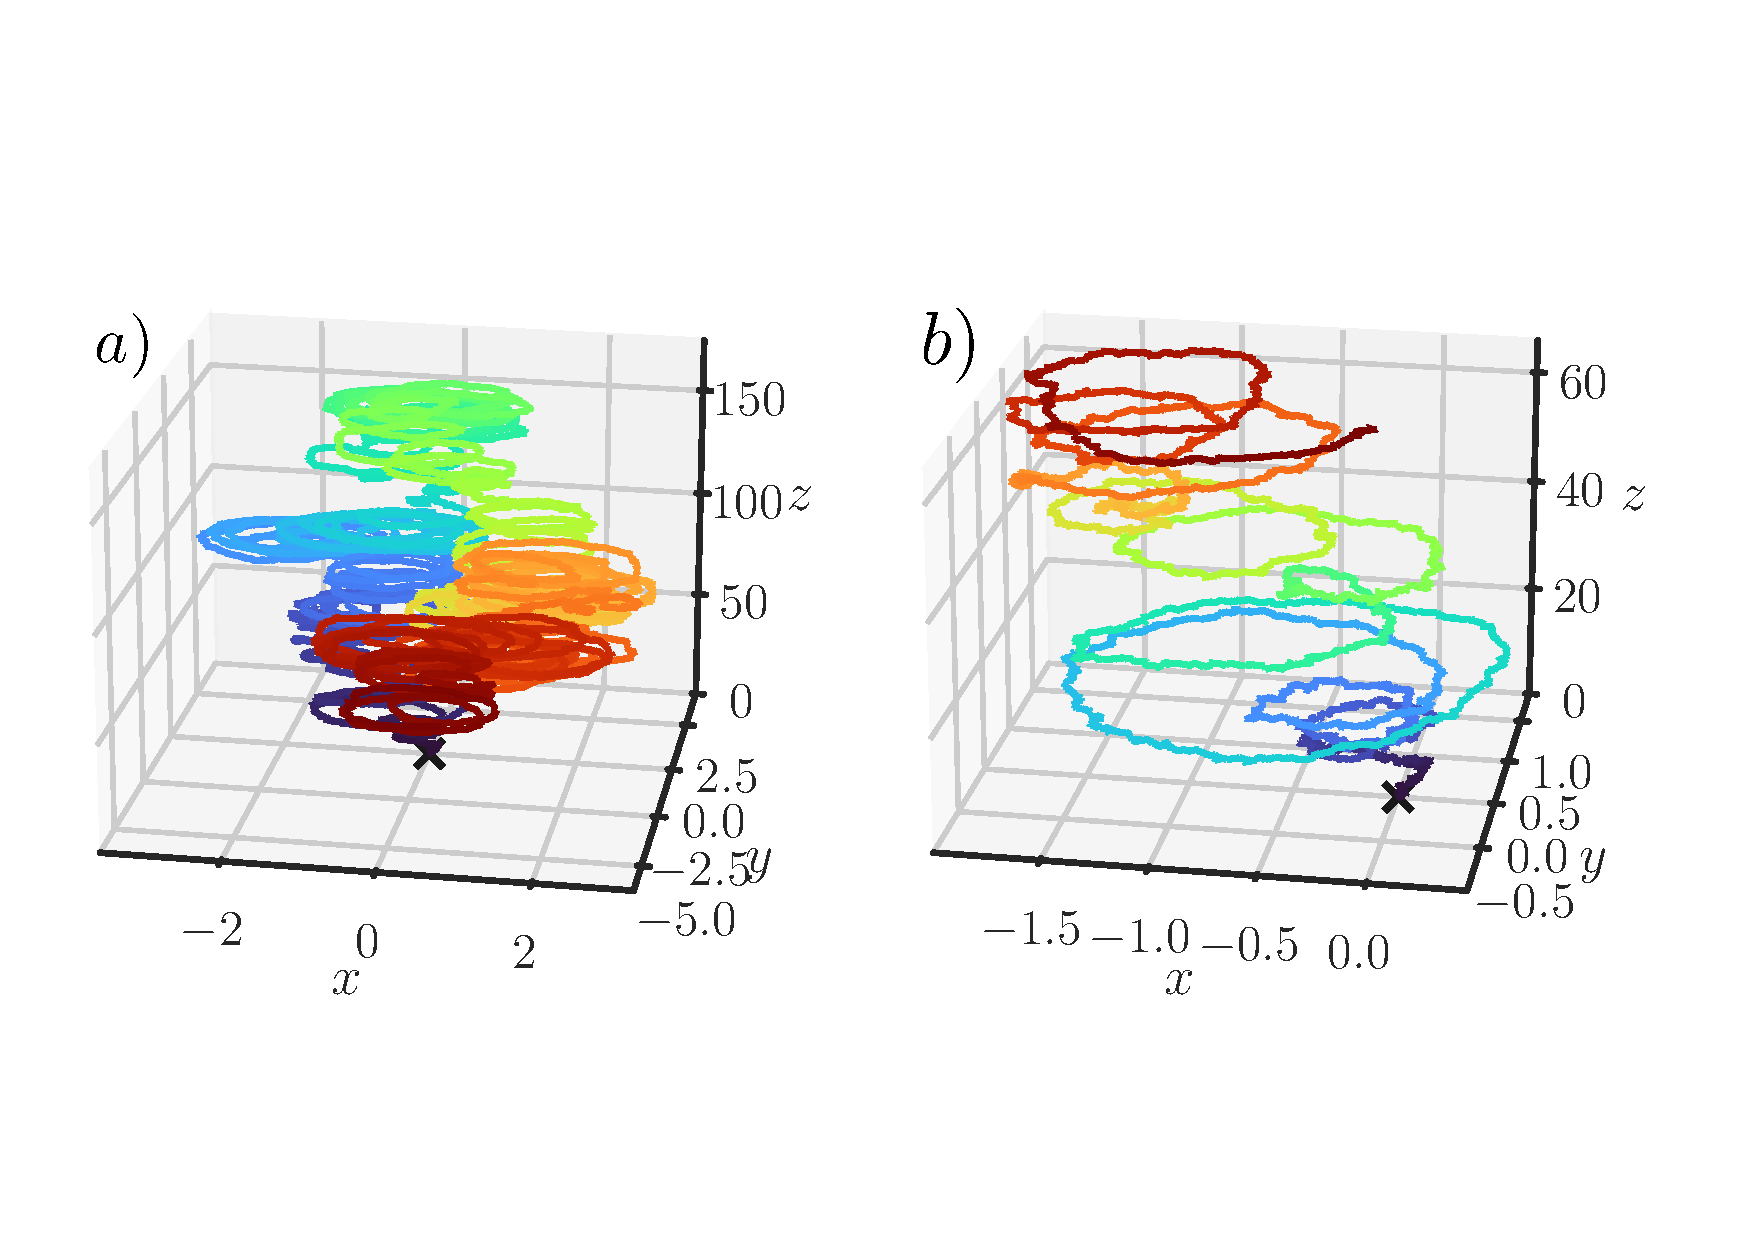
\includegraphics[width=1\textwidth]{figures/chapter5/helical.pdf}
    \caption[Simulation of a chiral ABP in 3D.]{Simulated trajectories from the discretised Eqs. \ref{3d_helical}. \textbf{a)} Full trajectory for $n_\mathrm{steps}=80000$, $\Delta T = 0.01$, $D_\mathrm{T} = 0.005$, $D_\mathrm{R} = 0.01$, $v = 1.0$, $\boldsymbol\Omega = 1.0$ and $\omega = \frac{\pi}{12}$. All units are in simulation units. }
    \label{Traj_helical}
\end{figure}


\subsection{Run-and-tumble}

\subsection{Other conventional methods for swimmer modelling}
The models I presented so far describe active matter through an ensemble of reduced sets of degrees of freedom. Therein, the swimmer is treated either as a point-like particle through its leading far-field hydrodynamic signature. Though minimal, these methods can be extremely efficient in terms of computation cost. In the next section, I present a case study where complex swimmers interact with a flow and two boundaries using these techniques and recover the correct behaviour observed in experiments. However, these more elementary techniques do not fully resolve the finite swimmer size, surface motion, full lubrication forces, or detailed flow structures that become important when swimmers come close to one another or to a boundary.

A first step is to represent the swimmer as a finite-size body with surface activity. The classical example is the squirmer model introduced by James Lighthill in 1952 \cite{lighthill1952squirming} but refined by Blake in 1971 \cite{Blake_1971}, in which a spherical particle swims by imposing a tangential slip velocity on its surface. The propulsion mechanisms are then modeled through the flow generated at the swimmer's boundaries. It is then possible to recover different swimmer behaviours (Shaker, pusher, puller, etc.) by tweaking the system's parameters. This model can be implemented in numerical methods such as the RigidMultiblobWalls method I describe in Chapter 2 to model complex, active bodies in a fluid. 

More resolved approaches include solving the fluid, such as boundary-element, immersed-boundary, multiparticle collision dynamics, or lattice-Boltzmann methods. These methods compute the fluid flow around the swimmer and can incorporate complex swimmer shapes, deformable boundaries, confinement, or no-slip walls. They are much more computationally demanding, but they provide access to regimes where the point-particle approximation breaks down.

Active-matter models thus span a full hierarchy of descriptions. Point-particle models are well suited to identify generic non-equilibrium mechanisms, and finite-size and hydrodynamically resolved models are necessary when near-field interactions, confinement, or details in the propulsion mechanism are in control of the dynamics.




\section{Active Brownian Particles in fluid flows}

\subsection{Context}
In Chapter 4, I introduce the notion of Taylor-Aris dispersion. While general Taylor-Aris dispersion has previously been developed theoretically for biased swimmers, gyrotactic microorganisms and active Brownian particles, our study provides an experimental realization with living \emph{Chlamydomonas reinhardtii} in a confined, sinusoidal Poiseuille flow. By combining single-cell tracking, Langevin simulations and moment analysis, we show here that the longitudinal dispersion coefficient increases with oscillatory flow amplitude and period and follows a generalized Taylor–Aris description for active swimmers.

\subsection{Chlamydomonas reinhardtii as a model swimmer}

A particularly convenient experimental model of a biological microswimmer is the unicellular green alga \emph{Chlamydomonas reinhardtii} (Fig. \ref{chlamy_img}). This alga is roughly spherical, micrometric-sized, and swims by beating its two anterior flagella in a breaststroke-like motion. It is also able to sense ambient light with photoreceptive apparatus akin to an eye. Depending on light nature and intensity as well as physiological conditions, the alga is then able to modify the beating of its flagella to steer towards or away from stimuli. Because of this simple geometry and well established and studied behaviour, \emph{Chlamydomonas} has become a standard model system for active matter in fluids. From a physics perspective, it is sufficiently simple to be idealized as an active particle using models we described above, yet sufficiently rich to show rich biological capacities like flagellar synchronization, phototaxis, rheotaxis, gliding, cell-body rotation and hydrodynamic interactions with boundaries or external fluid flows. For all these reasons, \emph{Chlamydomonas reinhardtii} is our organism of study for the remainder of this Chapter.

\begin{figure}
    \centering
    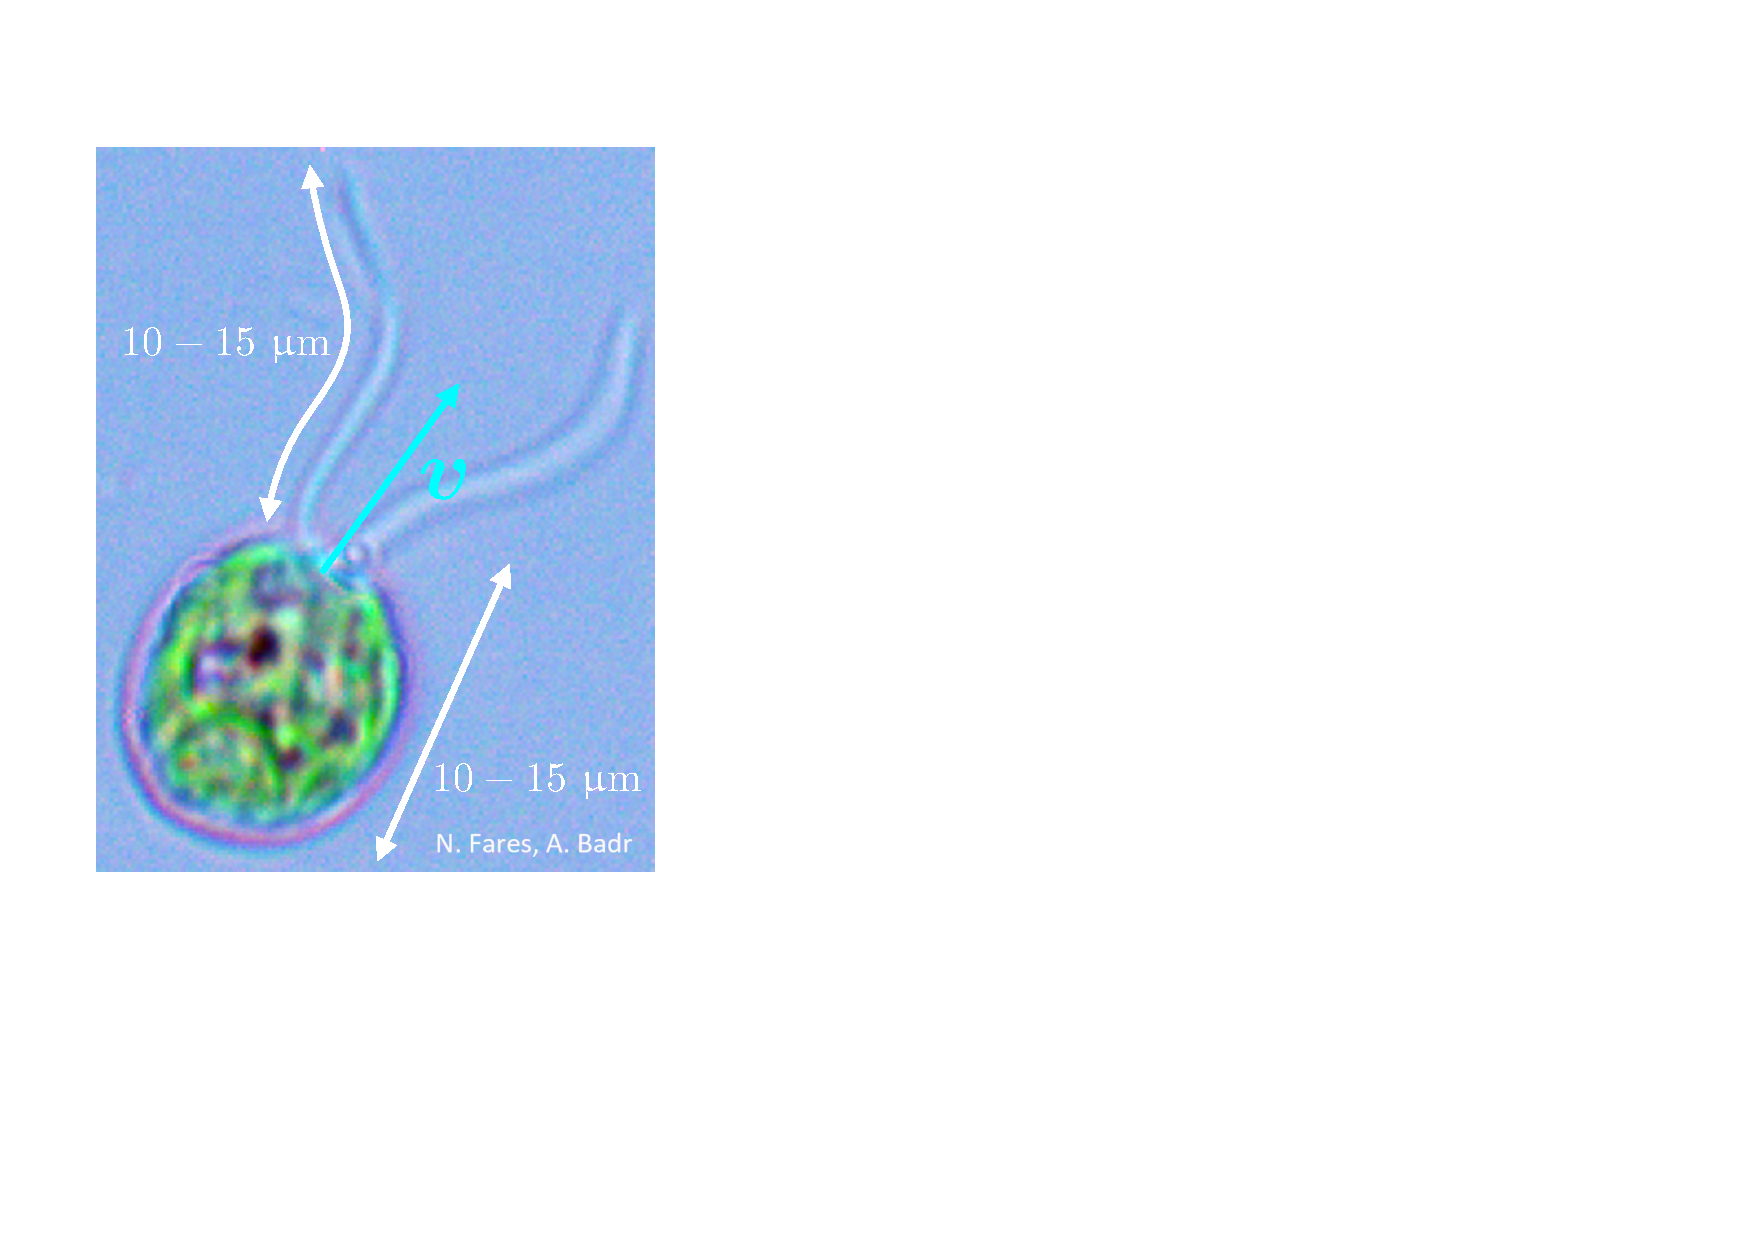
\includegraphics[width=.4\textwidth]{figures/chapter5/chlamy.pdf}
    \caption[Experimental setup for the study of Active Taylor Dispersion.]{Photograph of a \emph{Chlamydomonas reinhardtii} alga taken by Ahmad Badr and Nicolas Fares in our experimental rooms. The body and the flagella each measure about $10 \upmu \mathrm{m}$. The alga also features an eyespot which allows it to sense incoming light and adapt.}
    \label{chlamy_img}
\end{figure}



\subsection{Experimental setup}

We create a microfluidic channel using soft lithography on a PolyDimethylSiloxane (PDMS) chip. The channel has dimensions $(L, W, H) =  (88 \mathrm{mm}, 180 \upmu \mathrm{m}, 100 \upmu \mathrm{m}$), with $W$ the width, $H$ the height and $L$ the length of the channel (Fig. \ref{ExperimentalSetup}). The streamwise direction is defined along $\vec{e_x}$. The cell is then slowly filled with a dilute suspension of \emph{Chlamydomonas reinhardtii} to ensure negligible interaction between individual algae. We suppress phototacic response of the algae by filtering out light wavelength save for red. 

\begin{figure}
    \centering
    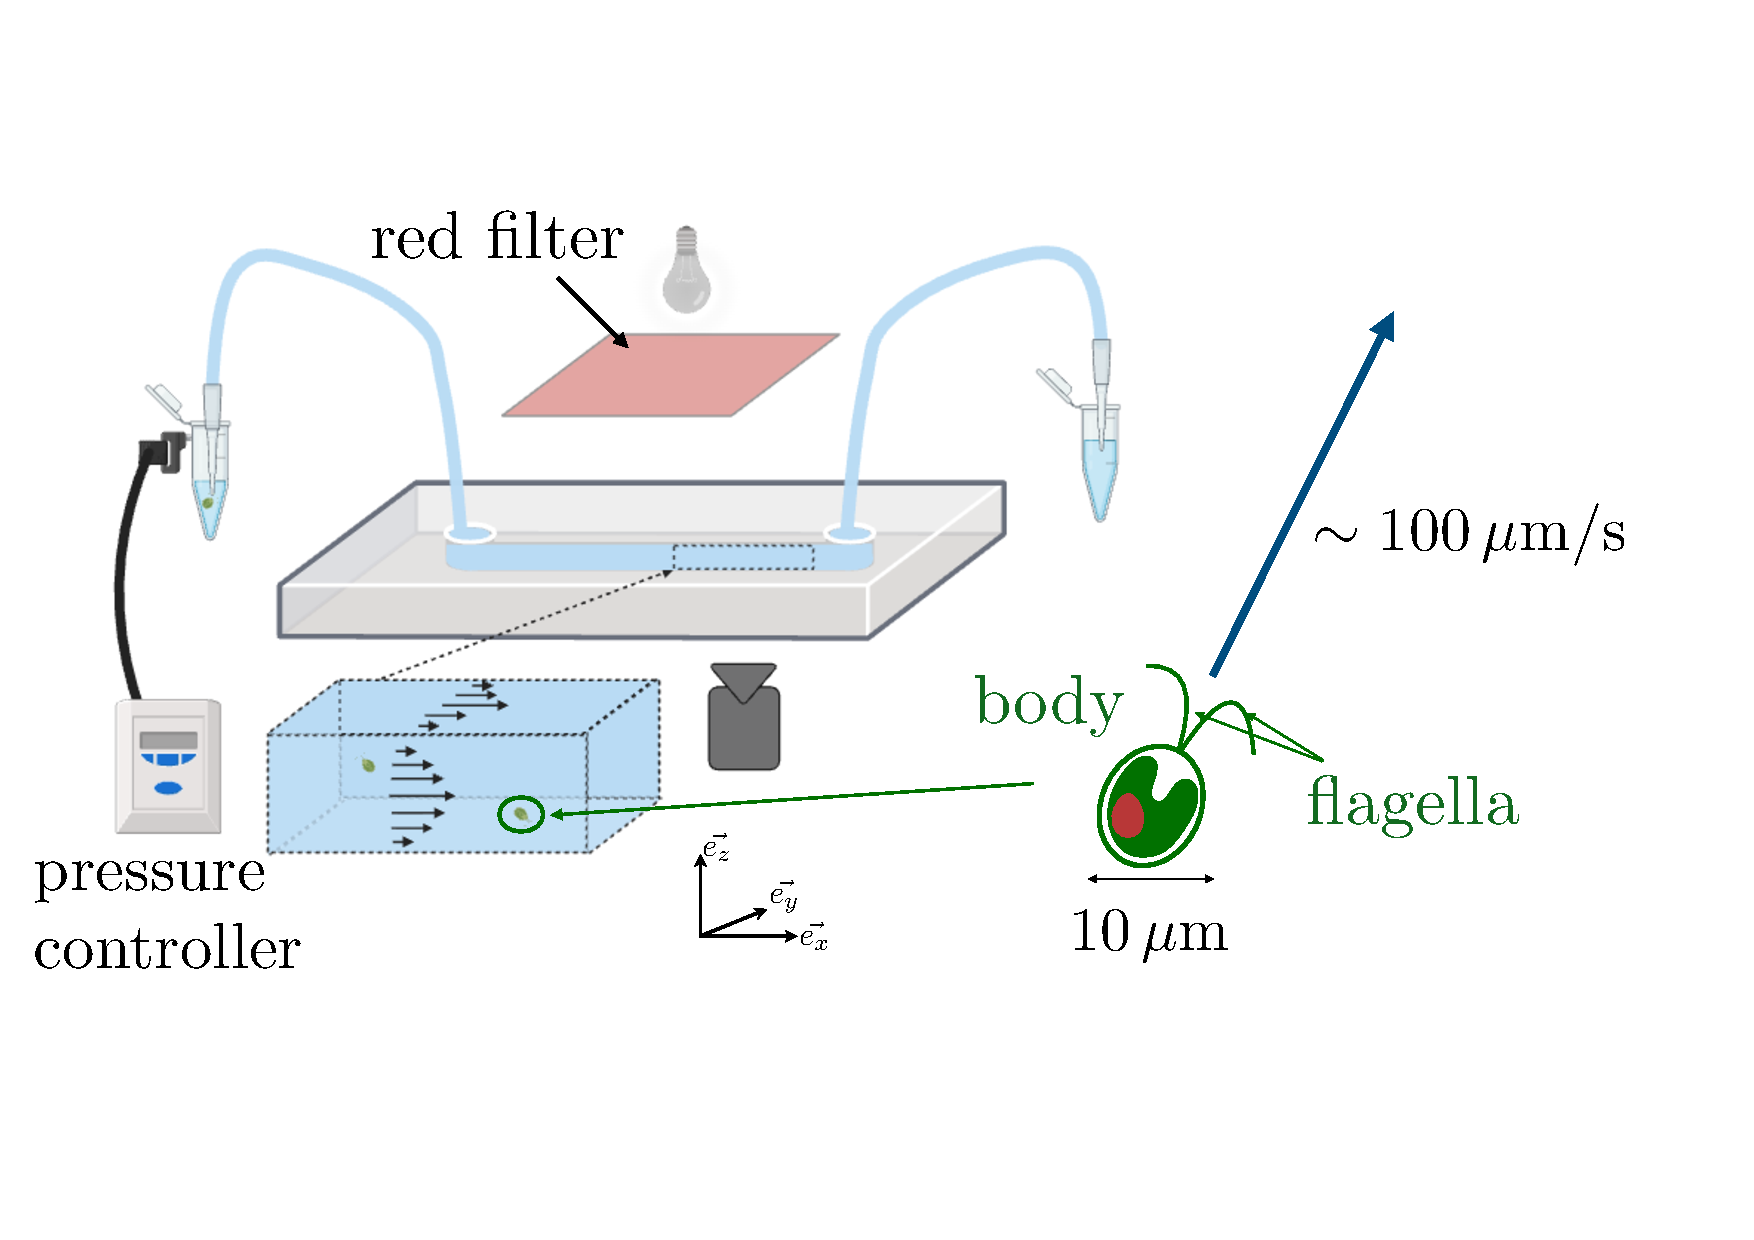
\includegraphics[width=1\textwidth]{figures/chapter5/experimental_setup.pdf}
    \caption[Experimental setup for the study of Active Taylor Dispersion.]{Schematic representation of the experimental setup for Active Taylor-Aris dispersion. A suspension of microswimmers is injected in a rectangular microchannel of width $W$, height $H$ and length $L$. An oscillating flow is imposed in the microchannel using a pressure controller at one end, whereas pressure is maintained constant on the other end with a reservoir. Swimmers are illuminated with a red-filtered light, and imaged with a high-framerate camera through an objective. }
    \label{ExperimentalSetup}
\end{figure}



A pressure controller is plugged at one end of the channel, on the entry point. On the exit point, constant pressure is maintained by a hydrostatic bath. We input a controlled pressure, which can be modulated by a sinusoid using the pressure controller. The pressure difference between the entry and exit points launches the flowing of the suspension inside the microchannel. The fluid velocity is given by:

\begin{equation}
    \vv{u}(y, z, t) = \frac{\Delta P}{R_\mathrm{h}} f (y ,z) \sin \left( \frac{2 \pi t}{T} + \phi_0\right) \vv{e_x}~,
    \label{fluidvelexp}
\end{equation}
where $\Delta P$ is the pressure difference between the amplitude of the pressure controller and the hydrostatic bath, $R_\mathrm{h}$ is the hydraulic resistance of the channel, $T$ is the pressure oscillation period, and $\phi_0$ is a phase at origin, and $f(x, y)$ is the cross-sectional profile, which in a quasi two-dimensional limit is expressed $f(y) = 4 \left( \frac{y}{W} \right) \left(1 - \frac{y}{W}\right)$. Because the channel is sufficiently narrow and our observations flatten out the $z$ coordinate, we use this expression of $f$ as our approximation for the study.




We then image the channel from the top, over the $z-$plane. We record frames for 200 s at 40 frames per second. We then link individual trajectories using a linking algorithm, and only keep trajectories which last for more than 20 s in the field of view of the camera for treatment. The oscillatory flow has the advantage of forcing the algae into the field of view for longer durations (Fig. \ref{ExperimentalTraj}).

The treatment of a single trajectory then involves demodulating the signal from the oscillatory signature of the flow velocity, assuming that the position of an alga in time along the $x-$axis can be expressed as

\begin{equation}
    x(t) = \hat{x(t)} + A[y(t), t] \cot \left( \frac{2 \pi t}{T}\right)~,
\end{equation}
where $A[y(t), t]$ is an unknown function, and $\hat{x(t)}$ is the position of the alga in the flow's comoving frame. 

\textcolor{blue}{HERE}



\begin{figure}
    \centering
    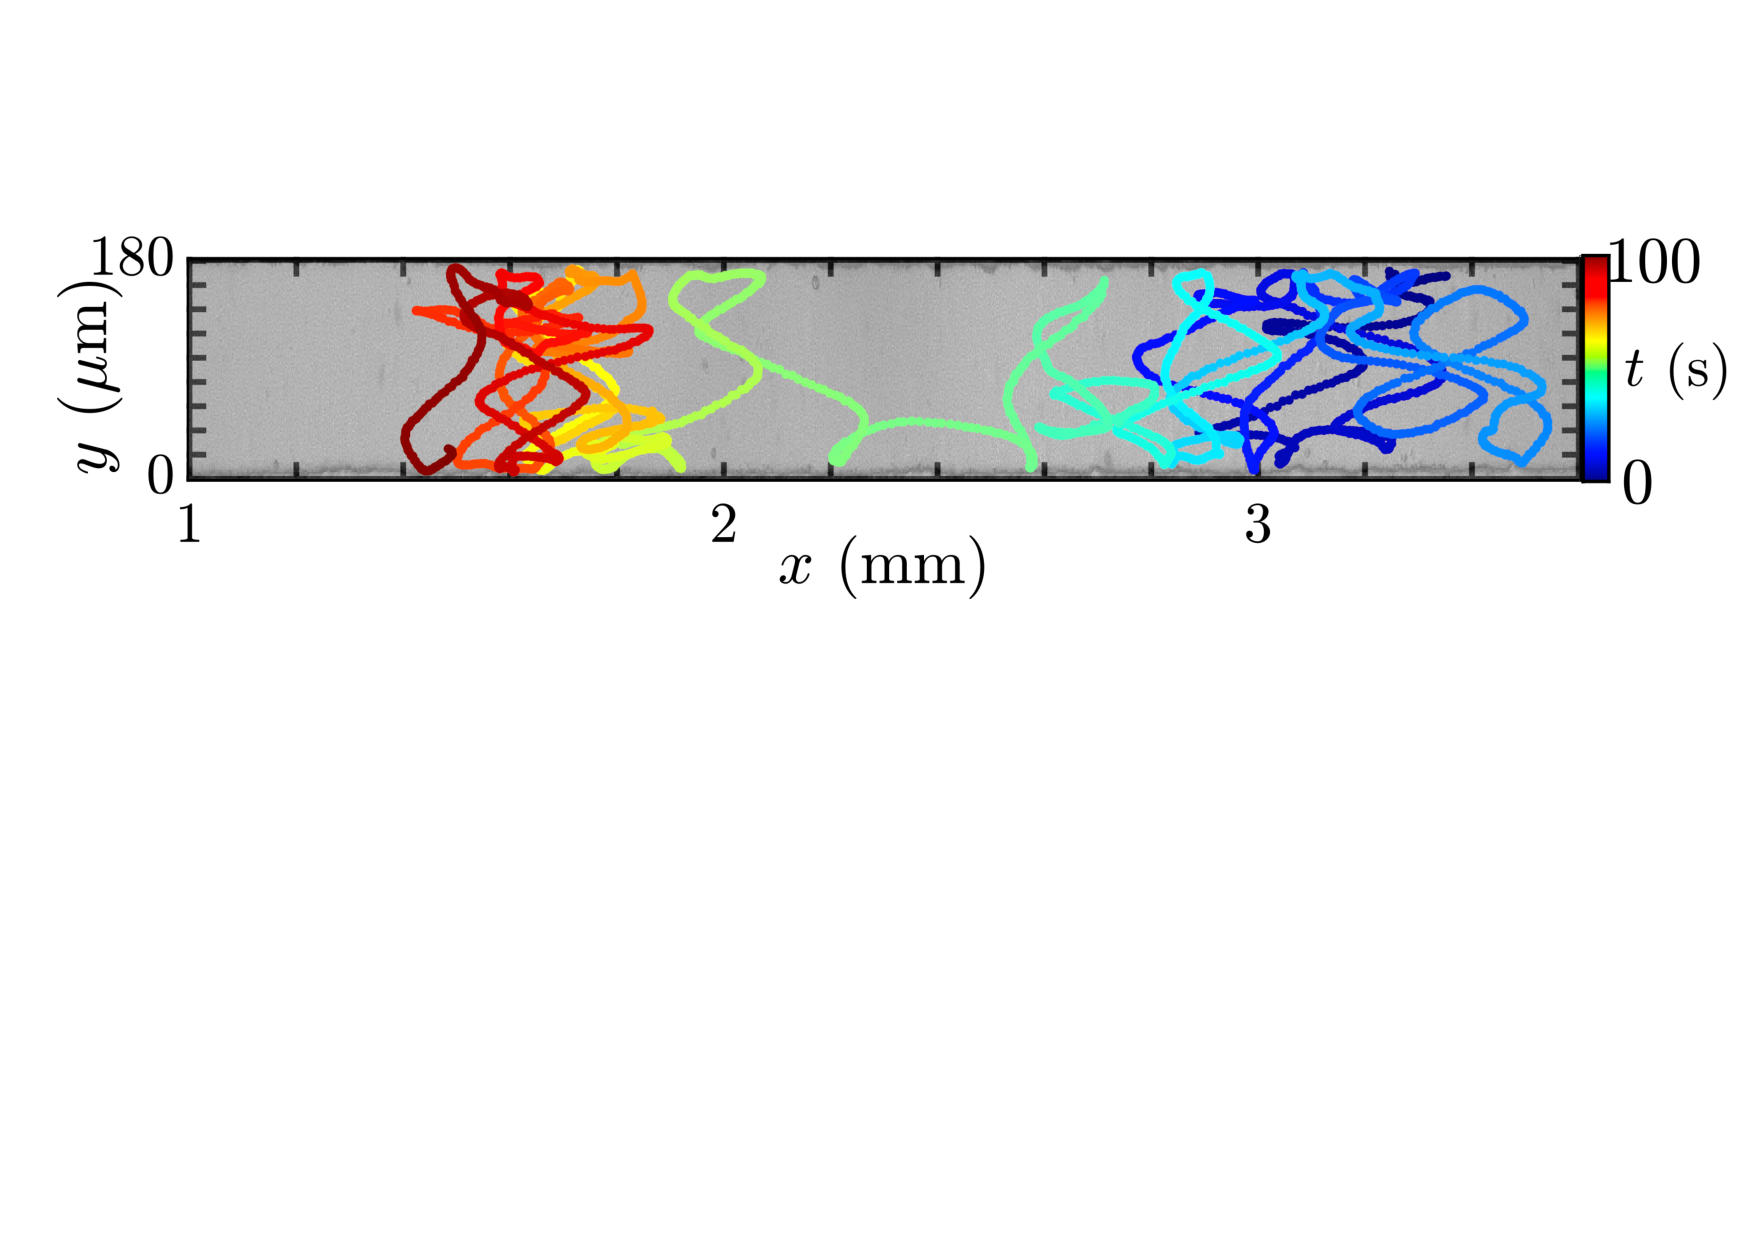
\includegraphics[width=1\textwidth]{figures/chapter5/exp_traj_rainbow.pdf}
    \caption[Experimental trajectory of a \emph{Chlamydomonas reinhardtii} in an oscillating Poiseuille flow.]{Typical experimental trajectory of a \emph{Chlamydomonas reinhardtii} in an oscillating flow. The colormap corresponds to elapsed time. }
    \label{ExperimentalTraj}
\end{figure}



\subsection{Numerical model}


\begin{align}
    \frac{\mathrm{d}x}{\mathrm{d}t} & = V_0 \cos [\phi(t)] + \sqrt{2D_0} \xi_x + u(y, t)~, \\ 
    \frac{\mathrm{d}y}{\mathrm{d}t} & = V_0 \sin [\phi(t)] + \sqrt{2D_0} \xi_y~, \\
    \frac{\mathrm{d}y}{\mathrm{d}t} & = \frac{1}{2} \omega(t) + \sqrt{2D_0} \xi_\phi~,
\end{align}
\begin{figure}
    \centering
    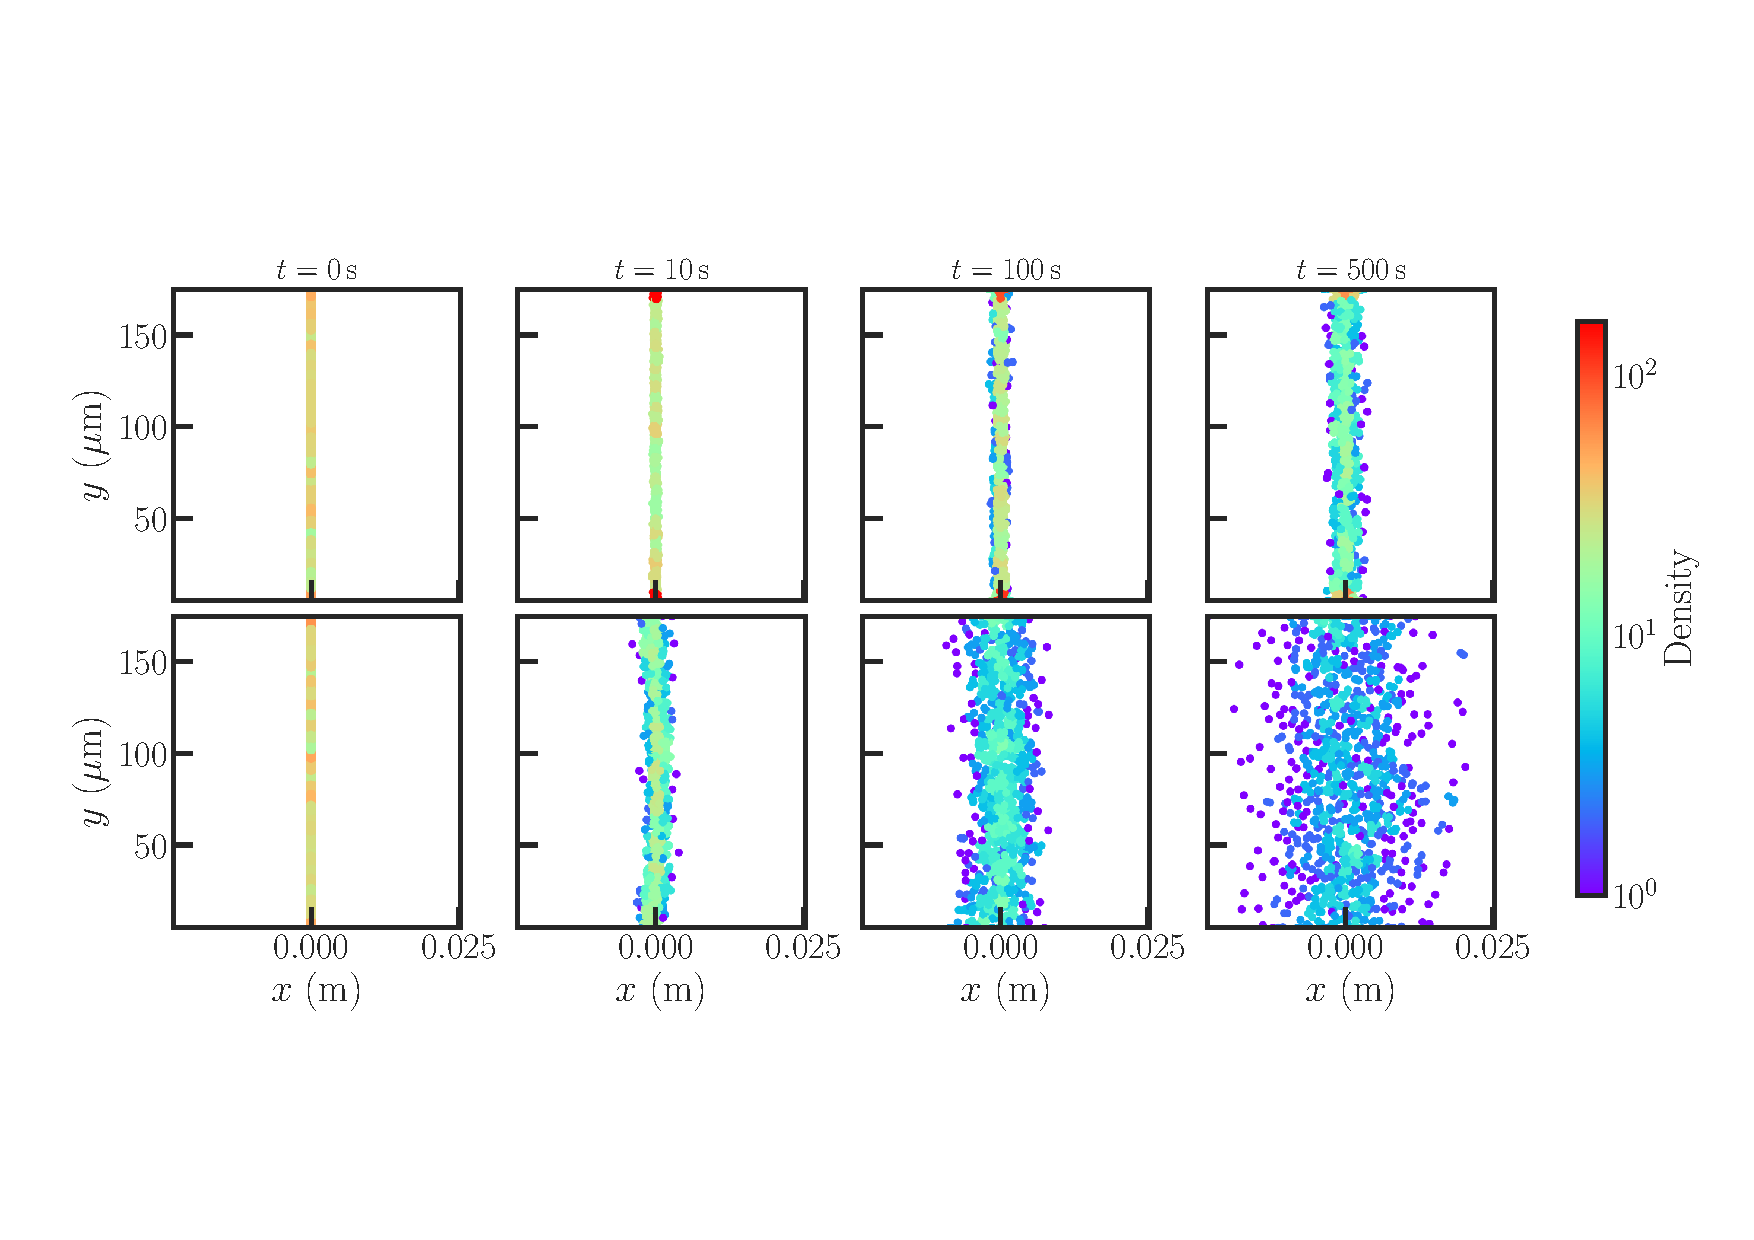
\includegraphics[width=1\textwidth]{figures/chapter5/numtraj1.pdf}
    \caption[]{}
    \label{NumTraj1}
\end{figure}

\begin{figure}
    \centering
    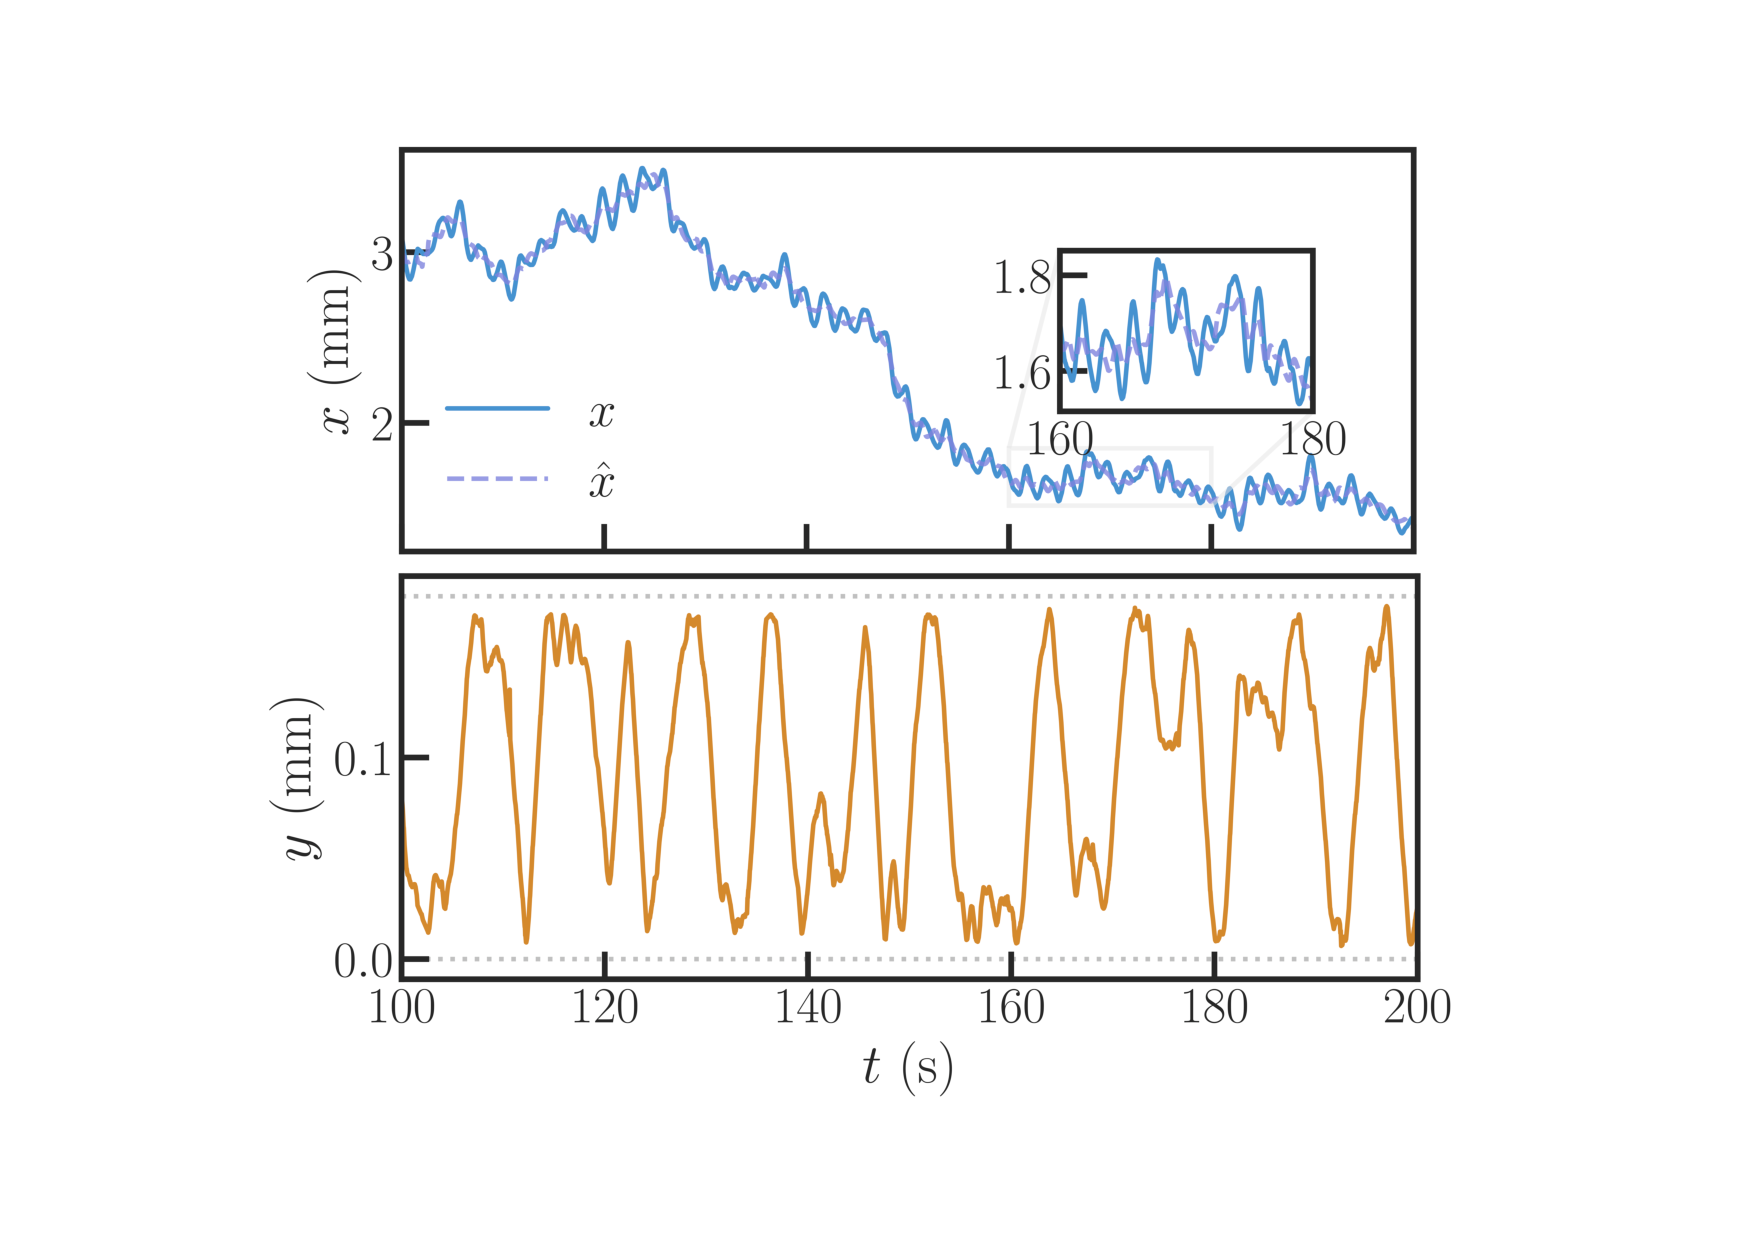
\includegraphics[width=1\textwidth]{figures/chapter5/numtraj2.pdf}
    \caption[]{}
    \label{NumTraj2}
\end{figure}




\subsection{Results}



\begin{figure}
    \centering
    
\includegraphics[width=1\textwidth]{figures/chapter5/MSD2.pdf}
    \caption[]{}
    \label{MSDpeclet}
\end{figure}

\begin{figure}
    \centering
    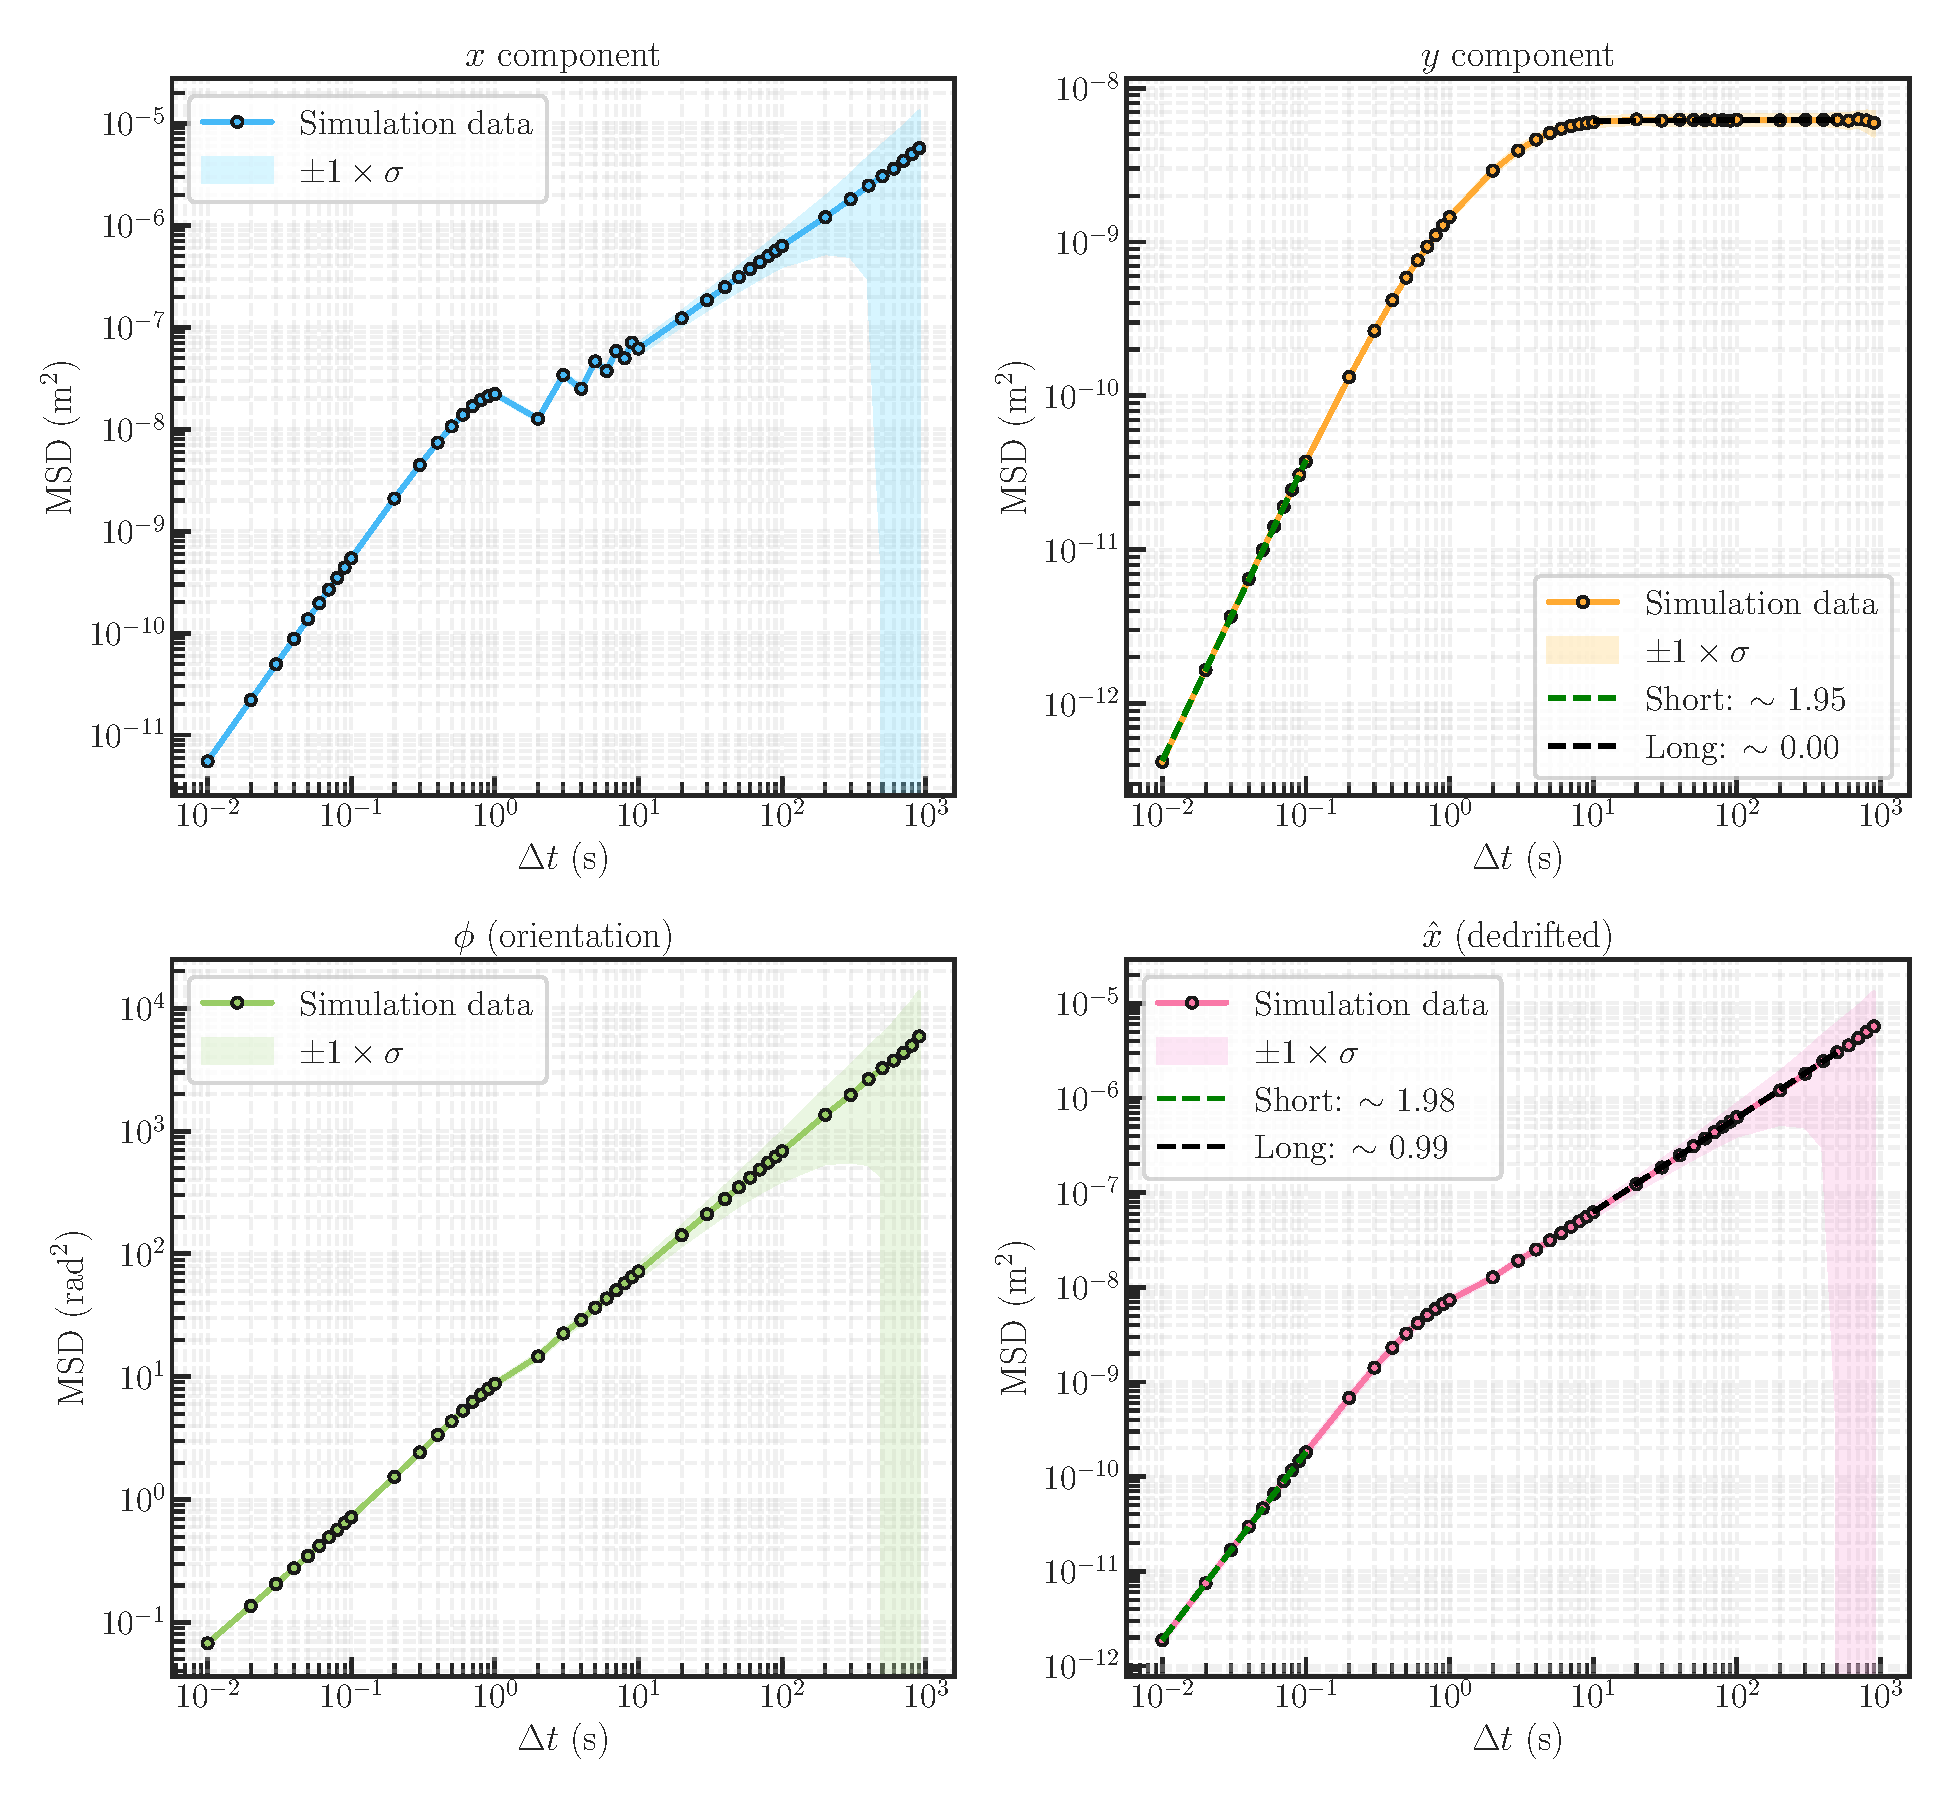
\includegraphics[width=1\textwidth]{figures/chapter5/N_1000000-tau_0.001-R_5e-06-H_0.0001-eta_0_0.001-kbT_4.141947e-21-D_r_3.35-v_0.0001-T_2.0-delta_P_9.943020230137991-L_0.088-W_0.00018-oscillations_True-N_trajectories_100-Job_ID_10_0.pdf}
    \caption[]{}
    \label{MSDfits}
\end{figure}

\begin{figure}
    \centering
    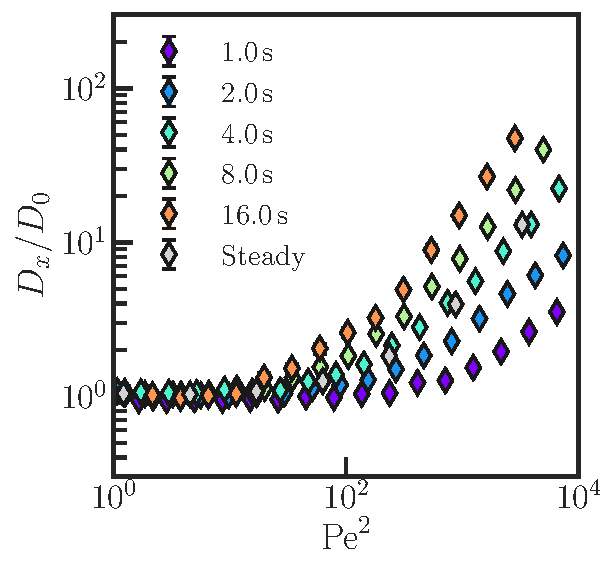
\includegraphics[width=1\textwidth]{figures/chapter5/dxd0_thesis.pdf}
    \caption[]{}
    \label{dxd0}
\end{figure}

\begin{figure}
    \centering
    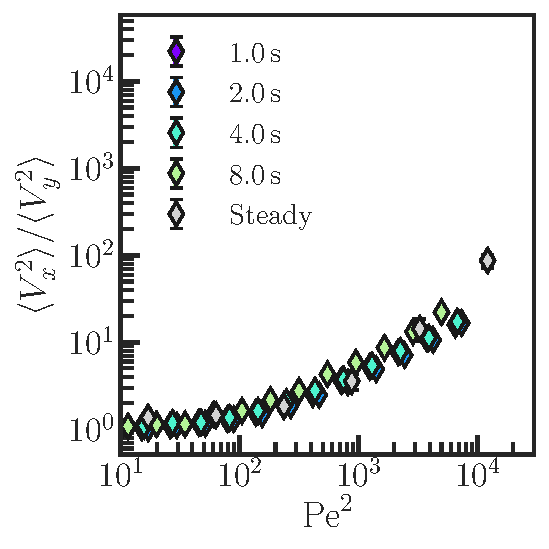
\includegraphics[width=1\textwidth]{figures/chapter5/vxvy_thesis.pdf}
    \caption[]{}
    \label{vxvy}
\end{figure}


\section{Conclusion and perspectives}



\section{Take-home messages}